\documentclass[fleqn,10pt]{olplainarticle}
% Use option lineno for line numbers 

\usepackage[parfill]{parskip}
\usepackage[innertopmargin=0.05cm]{mdframed}
\usepackage{blindtext}
\usepackage{geometry}
 \geometry{
 a4paper,
 total={170mm,257mm},
 left=20mm,
 top=20mm,
 }

\graphicspath{ {./../../Plots} {./Figures} }

\begin{document}

\section{Background}

\subsection{Mismatch Repair (MMR) System}

The MMR system is one of the many evolutionarily conserved pathways involved in the repair and maintenance of DNA. Specifically, MMR recognizes mismatched bases and insertion/deletion (indel) loops in newly synthesized DNA, for example during DNA replication or recombination. It acts in a strand-specific manner, triggering the degradation of the error-containing region in the daughter strand, allowing the cell to "try again" by resynthesizing the degraded DNA.

In humans, the protein MSH2 pairs with MSH6 to form the primary error-recognition complex of the MMR system. Similarly, MLH1 partners with PMS2 to create an endonuclease complex. Once an error is identified, the MLH1-PMS2 complex is recruited and activated by the MSH2-MSH6 complex, with additional assistance from cofactors such as PCNA and RFC. Upon activation, MLH1-PMS2 introduces multiple nicks on the 5' side of the error in the daughter strand. Exo1 is then recruited to these nicks, where it degrades the strand in the direction of the error. Subsequently, DNA polymerase $\delta$ or $\epsilon$ resynthesizes the excised segment, and the repair process is completed by DNA ligase I, which seals the strand.

The MMR system involves numerous other proteins, including alternative heterodimer combinations (Figure 1). While these heterodimers are less well-characterized, they are generally less active and exhibit overlapping functionality with the primary complexes described above, making them largely redundant.

\begin{figure}[!h]

\centering
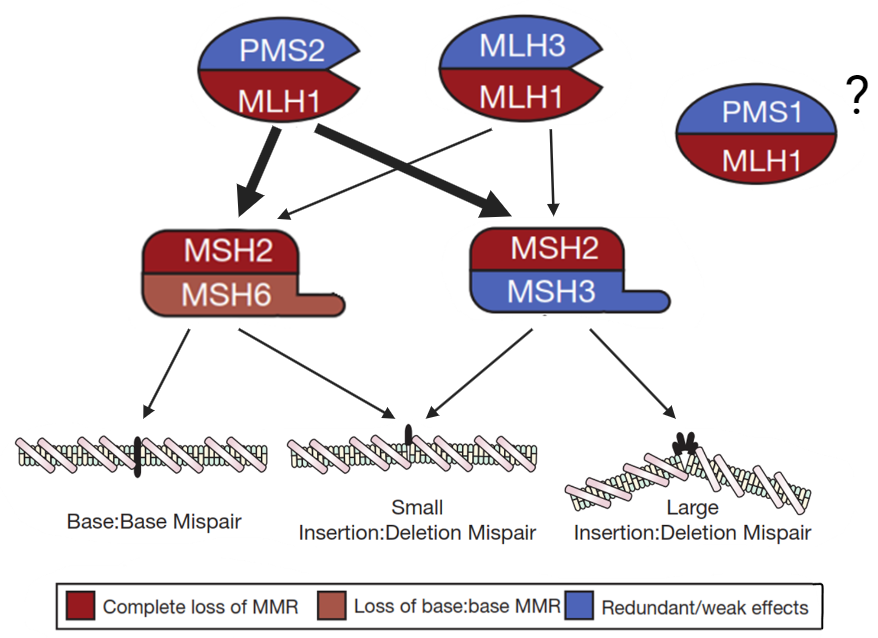
\includegraphics[scale=0.55]{MMR.png}
\caption{\textbf{Overview of the human MMR system}. MSH2 can also dimerize with MSH3 to form a separate error-recognition unit. These two units differ in terms of their binding affinities to different types of errors. Similarly, MLH1 can also dimerize with MLH3 and PMS1. MLH1-MLH3 can substitute for MLH1-PMS2 but plays a more minor role. On the other hand, not much is known about PMS1-MLH1. Color indicates effect of protein loss.}

\end{figure}

\subsubsection{Anti-mutagenic effect of MMR}

If left unrepaired, mismatches and indel loops may develop into base and indel mutations respectively during the next cell cycle. Thus, MMR minimizes the frequency of these mutations by preventing the formation of its precursors. Mutation or inactivation of key MMR genes (MLH1, MSH2, MSH6, PMS2) lead to an MMR deficient (MMRd) phenotype, which is characterized by elevated mutation rates. Indeed, MMRd mice had a significantly higher indel mutation rate (up to $\sim$72 fold in MLH1$^{-/-}$) compared to WT, MMR proficient (MMRp) mice, as determined by a supFG1 reporter assay.

[MMR in apoptotic response to mutagens, MMR in homeologous recombination]

%The MMR system is also able to recognize and bind mutagenic DNA lesions formed by alkylating agents, reactive oxygen species, UV radiation, etc... For example, alkylating agents are often used as chemotherapeutics and they work by inducing the formation of O$^6$-meG, which tends to mispair with thymine. This mismatch is recognized by the MMR system, triggering a cell cycle arrest / apoptotic cascade, preventing a GC $\rightarrow$ AT transition. Consequently, MMR deficient cancer cells are resistant, and may perhaps benefit from these agents. 

%The MMR system also restricts homologous recombination between divergent strands of DNA (homeologous recombination) by binding to mismatches formed during strand invasion and triggering heteroduplex rejection.

\subsubsection{Pro-mutagenic effect of MMR}
Although the primary role of MMR is anti-mutagenic, there are instances where it can contribute to mutagenesis, particularly in the context of trinucleotide repeat (TNR) expansions. For example, studies in Huntington's disease (HD) transgenic mice revealed that the expansion of CAG repeats (correlated with a more severe HD phenotype) was reduced in MSH2-deficient mice compared to wild-type counterparts.

Additionally, MMR overexpression was frequently observed in late-stage prostate cancer, where it correlated with poor prognosis and genomic instability phenotypes such as large-scale deletions. While this alone does not confirm a causal role for MMR function in driving genomic instability, experiments in yeast showing that co-overexpression of MSH2 and MSH6 induced similar genomic instability phenotypes may support this hypothesis.

\newpage

\subsubsection{MMR in Cancer Aetiology}
An increased mutational burden is a key driver of cancer initiation and progression, contributing to tumor heterogeneity and therapy resistance. Unsurprisingly, changes in MMR expression, in particular MMRd, can be seen across various tumor types. This is because MMRd cells are more prone to mutations, increasing their likelihood of becoming cancerous. The prevalence of MMRd varies widely across cancers, ranging from as low as $\sim$1\% (prostate, bladder, etc..) to as high as $\sim$15\% in colorectal (CRC) and $\sim$30\% in endometrial cancer (EC).

[MMRd can be sporadic or inherited (Lynch)]

[Differences MMRd tumors vs MMRp tumors]

[CMMRD]

%However, only three of the 15\% of MMRd tumors in CRC and 
%tumors have a sporadic origin (12). These tumors are mainly caused by biallelic hypermethylation of the MLH1 promoter, leading to epigenetic silencing (12). Biallelic somatic MMR mutations are also a possible cause but they are rare (12). Despite both sporadic and LS-related tumors in CRC and EC being MMRd, they behave quite differently. Morphologically, tumor lymphocyte infiltration (TILs), tumor cell de-differentiation, and presence of adenomas is more common in LS-related than sporadic MMRd CRC (13). TILs are also more common in LS-related EC (14). Additionally, sporadic MMRd CRC tends to occur in the proximal colon while there is no such preference in LS-related CRC (12).

\subsection{Lynch Syndrome}

Germline mutations in one of : MLH1, MSH2, MSH6, PMS2 (or more rarely a deletion in EPCAM which causes epigenetic silencing of MSH2) characterizes a heritable cancer predisposition disease known as Lynch syndrome (LS). LS patients are more susceptible to the MMRd phenotype since additional events, such as somatic mutations or promoter hypermethylation, can inactivate the remaining functional allele of the affected gene, a mechanism known as the "two-hit hypothesis." MLH1 and MSH2 defects are the most common in LS, accounting for 60-80\% of cases. Defects in these genes comes with the lifetime risk (by age 70) of $\sim$50\% for CRC and $\sim$40\% for EC. While other mutations are milder in effect ($\sim$10-20\% risk), it is still much higher than the general population risk of 2\% and 1\% respectively. 

LS is one of the most common hereditary cause of CRC predisposition, it has an estimated population prevalence of 0.3\%. Due to its hereditary nature, genetic counselling is relevant in LS. It is important to identify LS patients early on since preventative measures can be taken to reduce cancer incidence and mortality. For example, positive results have been shown for intensive colonoscopic surveillance and chemoprevention with aspirin. Furthermore, identifying LS patients facilitates cascade genetic testing in relatives, enabling early detection and intervention.

\subsection{MMRd detection \& Lynch Diagnosis}

MMRd detection in tumors is important since it serves as the initial step towards identifying LS patients. More generally, due to their distinct biological behavior, distinguishing between MMRd and MMRp tumors allows care-providers to make informed clinical decisions, for instance in the choice of therapy, and predicting prognosis, ultimately improving patient outcomes. 

Traditionally, there are two ways to detect MMRd : 

\begin{enumerate}

\item \textbf{Immunohistochemistry (IHC)}, which uses antibodies against the 4 major MMR proteins to measure their expression, a lack of which would suggest MMRd. However, mutations in MMR genes can lead to the production of nonfunctional proteins that remain antigenic, potentially resulting in false negatives. It is estimated that around 6\% of MMRd cases, particularly those related to MLH1, escape IHC detection due to this issue. 

\item \textbf{Microsatellite instability testing}. Microsatellites are genomic regions composed of short sequence motifs (1–6 bp) repeated in tandem. These regions are particularly prone to indel loop formations caused by strand slippage during DNA replication, resulting in an increased occurrence of mutant-length alleles—a phenomenon known as microsatellite instability (MSI). Normally, MSI is kept at low levels by the MMR system, but without it, indel mutations accumulate unchecked, leading to a significant increase in MSI. This sensitivity of microsatellites to MMR function forms the basis of MSI testing (see section 1.4)

\end{enumerate}

MSI testing and IHC are highly concordant (92-99\%). Using both tests in conjunction, almost 100\% of MMRd tumors can be identified. MMRd tumors can be further classified by their origin—either sporadic or hereditary (LS). This is done through germline sequencing of the MMR genes. 

[BRAF and MLH1 methylation analysis?]

[Functional MMR assays?]

%Other features suggestive of LS include a family history of CRC/EC and a diagnosis below the age of 50-60. Molecularly, the presence of either a somatic BRAF.1779T>A mutation or MLH1 promoter methylation is quite rare in LS (1.4\% and 6\% of LS cases in CRC), thus its presence is a strong negative predictor for LS. 

\subsection{MSI testing}

MSI testing involves PCR amplification and sequencing of specific microsatellite markers. The frequencies of the various length alleles are then compared between paired normal/tumor samples from the same individual. Alternatively, quasi-monomorphic microsatellite markers may be used. These are microsatellites whose major (also known as reference) allele is present with frequency $\geq$ 95\% in the population. This means that PCR on normal tissues is unnecessary since the reference allele is assumed to be the same as seen in a human reference genome library (hg19).

One significant challenge with MSI testing is that the PCR amplification step introduces additional indel mutations through the same "slippage" process that causes indels to occur naturally in vivo. This introduces a degree of noise in the PCR products, which is particularly concerning for data analysis involving rare ($<$1\% frequency) allelic variants, as it becomes difficult to distinguish true in vivo mutations from artefacts introduced during amplification.

The error rate per PCR cycle increases linearly with the number of repeat units in a microsatellite, making longer repeats more susceptible to errors. There is also a threshold repeat size, typically around 4–5 units depending on the sequence motif, below which PCR-induced errors are undetectable. Based on these observations, models of microsatellite mutation have been developed to predict and correct errors introduced during PCR amplification.

A more straight-forward approach to account for these errors is the use of unique molecular identifiers (UMIs)—short, random nucleotide sequences attached to individual DNA molecules prior to amplification. After sequencing, reads are grouped into "UMI families" based on their shared origin from the same template molecule. A consensus sequence is then derived for each family, typically by selecting the most common sequence, to represent the true allele. While this method effectively eliminates the majority of PCR-induced errors, it significantly reduces the number of reads available for analysis, and thus requires a high sequencing depth to be effective. Despite this, it has been explored as a reliable technique for more accurate microsatellite genotyping, particularly in forensic applications.

%\section{Methods}
%
%\subsection{Pre-processing}
%
%For each sample, PCR read counts were sorted into bins by marker and allele length. These allele lengths were standardized by taking the difference in length to the reference allele (as seen in the hg19 library). For example, the reference allele itself has length zero, a lbp deletion results in an allele of length -1, and so on. For example, reads from the marker LR52 with a 2bp deletion were placed into the "LR52(-2)" bin (this grouping is known as a marker-allele combination). 
%
%For each marker-allele combination, the allele frequency was determined by dividing the read count for that specific combination by the total read count across the marker. Additionally, the variant frequency (VF) was calculated as a similar measure, excluding the reference read count from the total marker read count (answers the question : how frequent is each mutant allele? i.e. it is the likelihood that a reference allele, once mutated, will result result in that particular variant). Unless stated otherwise, the frequencies used in the analysis refer to the standard allele frequencies, not the variant frequencies.

\section{Allele Frequency Analysis}

In an earlier study, we investigated differences in the frequency of different length alleles in MMRp and MMRd samples in CRC and EC (cite previous work?). In particular, the frequency of length alleles corresponding to deletions (-1, -2) are significantly higher in the MMRd group than the MMRp group as expected. Crucially, this pattern was not observed for the insertions, moreover our results seemed to suggest that the +1 allele is more frequent in the MMRp group instead. While this pattern was observed in both CRC and EC datasets, it was more clearly observed in CRC, which suggests tissue-specific differences.


%To do this, for each marker-allele combination, a ratio was calculated according to the following formula : 
%
%$$ r = \frac{x}{x+y} $$
%
%where $x,y$ are the median AF values for the particular marker-allele combination across the MMRp and MMRd samples respectively. 

The differing behaviour of insertion and deletion alleles in MMRp and MMRd samples challenges the assumption that the MMRd phenotype universally increases the frequency of all types of length mutations, including insertions. There are two possible explanations for this discrepancy :

\begin{enumerate}

\item \textbf{PCR errors}. The observed +1 alleles may simply result from PCR sequencing artifacts, particularly given their low frequencies (<1\%), which make them difficult to differentiate from PCR-induced noise. Furthermore, the larger initial "pool" of reference (zero-length) alleles in the MMRp samples could serve as a source for +1 allele generation through during the PCR process. This could explain the higher frequency of +1 alleles observed in the MMRp samples.

\item \textbf{A normal function of MMR}. As previously discussed, MMR can have pro-mutagenic effects, particularly in the context of TNR expansion. Thus, it is possible that MMR activity directly contributes to the higher +1 allele frequency observed in the MMRp samples.

\end{enumerate}

Assuming the first hypothesis is true, then the +1 allele frequency could potentially be used to estimate the PCR error rate, this can help further normalize the dataset. Assuming the second hypothesis is true, then the +1 allele frequency can be used as a predictor for the level of MMR function.

\subsection{Replication of Previous Result}

To reconfirm our previous observation, that the +1 allele frequencies are higher in MMRp than MMRd samples, we checked to see if this result can be replicated in other datasets as well, these include : 2 new CRC datasets (CRC1, CRC2) and a CMMRD dataset. Importantly, the CMMRD dataset gives us a look into how MMRd affects MSI in a non-tumor environment, free from effects such as homogeneity from clonal expansion, etc...  

\newpage

To achieve this, frequencies of the +1 allele were compared between the MMRp and MMRd groups for each marker using a two-tailed Mann-Whitney U test, crucially this allows us to check for marker-specific differences, something that was not done in the previous study. Additionally, a directional AUC was calculated, where higher AUC values indicate greater frequencies in the MMRd group, and lower values suggest higher frequencies in the MMRp group. This analysis was repeated for the -2, -1, and 0 length alleles (Figure 2).


\begin{figure}[h]
\includegraphics[scale=1]{"Figure1.png"}
\caption{Plot showing markers and the degree in which allele frequency significantly differs between MMRp and MMRd groups in each of the 6 datasets. Each marker is represented as a point, with color to indicate significance (blue : no significance, yellow : slight significance, red : very significant), and AUC to indicate directionality (AUC $<$ 0.5 : frequencies are higher in MMRp group, AUC $>$ 0.5 : frequencies are higher in MMRd group).}
\end{figure}

These results are in general agreement with our previous observation. The same pattern was successfully replicated in the new CRC datasets, but not in the CMMRD dataset. The behaviour of each allele is, in general, consistent between datasets with exception to the +1 allele which has a strong MMRp tendency in the CRC datasets, with this tendency being weaker in the EC datasets, and nonexistent in the CMMRD dataset. 

It is also interesting to note that for 1 particular marker (DEPDC2), the +1 allele has the same behaviour as the deletion alleles, that is, being more frequent in the MMRd group. This is the sole significant (yellow) marker in the "right" (AUC$>$0.5) direction for the +1 allele in all of the datasets.

Since datasets of the same condition behave similarly, this justifies their merging in future analysis.

\newpage


\subsection{With UMI}

Next, we performed the same analysis using consensus sequence obtained from UMI groupings (D1, D2) to check if PCR error correction has any effect on the patterns observed in the raw data, which still contains PCR noise (Figure 3)

\begin{figure}[h]
\includegraphics[scale=1]{"Figure2.png"}
\caption{Placeholder}
\end{figure}

The allele that is most significantly affected by the UMI grouping process is the +1 allele. This is unsurprising as, being a rare variant, the +1 allele is more likely to be affected by PCR noise. While this observation supports the PCR error hypothesis, it remains to be shown why this pattern is more readily observed in some datasets (CRC) but not others (CMMRD). (different tumor/tissue type have different PCR error rates??)

Markers in the +1 allele shifted to the right when UMI groupings were introduced, essentially reversing the previously observed pattern. This indicates that the "true" behavior of the +1 allele is probably closer to that of the deletion alleles than our initial data suggests.

\end{document}
